\subsection{Mirrors Re-coating}


Add mirror pieces to cover gaps





cyl, ell, parabolic.




\paragraph{Mirrors Reflectivity Measurements}

\begin{figure}[hbt]
\centering
	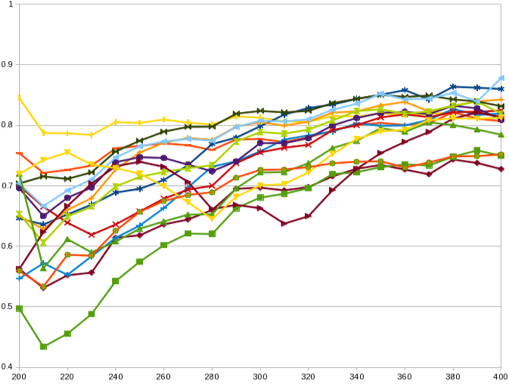
\includegraphics[width=1.0\columnwidth,keepaspectratio]{img/mirrorsReflectivityBefore.png}
	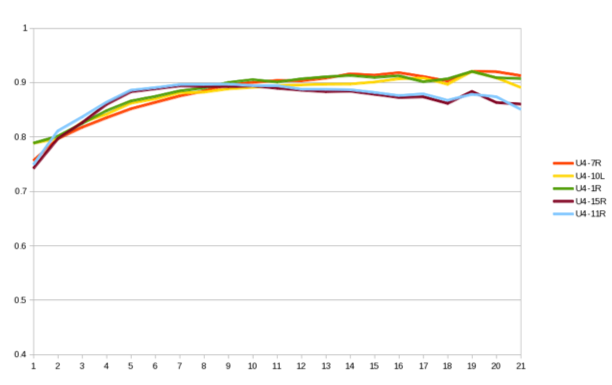
\includegraphics[width=1.0\columnwidth,keepaspectratio]{img/mirrorsReflectivityAfter.png}
	\caption{Average number of reflections calculated from simulations studies.}
	\label{fig:reflectivityFixed}
\end{figure}



\paragraph{Mirrors Alignment}



\begin{figure}[hbt]
\centering
	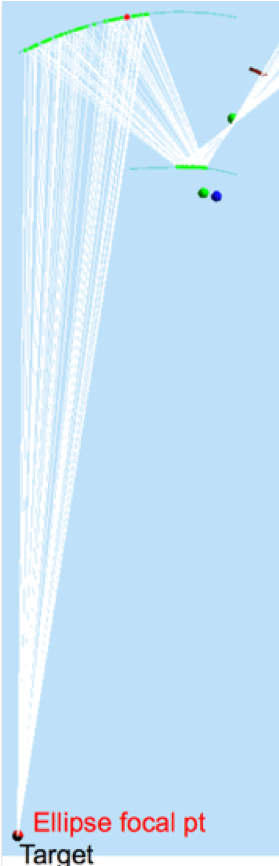
\includegraphics[width=1.0\columnwidth, height=0.5\textheight]{img/mirrorAlignmentSimulation.png}
	\caption{Average number of reflections calculated from simulations studies.}
	\label{fig:alignmentSimulation}
\end{figure}
